
\documentclass[a4paper,11pt]{article}
\usepackage[a4paper, margin=8em]{geometry}

% usa i pacchetti per la scrittura in italiano
\usepackage[french,italian]{babel}
\usepackage[T1]{fontenc}
\usepackage[utf8]{inputenc}
\frenchspacing 

% usa i pacchetti per la formattazione matematica
\usepackage{amsmath, amssymb, amsthm, amsfonts}

% usa altri pacchetti
\usepackage{gensymb}
\usepackage{hyperref}
\usepackage{standalone}

% imposta il titolo
\title{Appunti Comunicazioni Numeriche}
\author{Luca Seggiani}
\date{2026}

% imposta lo stile
% usa helvetica
\usepackage[scaled]{helvet}
% usa palatino
\usepackage{palatino}
% usa un font monospazio guardabile
\usepackage{lmodern}

\renewcommand{\rmdefault}{ppl}
\renewcommand{\sfdefault}{phv}
\renewcommand{\ttdefault}{lmtt}

% disponi il titolo
\makeatletter
\renewcommand{\maketitle} {
	\begin{center} 
		\begin{minipage}[t]{.8\textwidth}
			\textsf{\huge\bfseries \@title} 
		\end{minipage}%
		\begin{minipage}[t]{.2\textwidth}
			\raggedleft \vspace{-1.65em}
			\textsf{\small \@author} \vfill
			\textsf{\small \@date}
		\end{minipage}
		\par
	\end{center}

	\thispagestyle{empty}
	\pagestyle{fancy}
}
\makeatother

% disponi teoremi
\usepackage{tcolorbox}
\newtcolorbox[auto counter, number within=section]{theorem}[2][]{%
	colback=blue!10, 
	colframe=blue!40!black, 
	sharp corners=northwest,
	fonttitle=\sffamily\bfseries, 
	title=~\thetcbcounter: #2, 
	#1
}

% disponi definizioni
\newtcolorbox[auto counter, number within=section]{definition}[2][]{%
	colback=red!10,
	colframe=red!40!black,
	sharp corners=northwest,
	fonttitle=\sffamily\bfseries,
	title=~\thetcbcounter: #2,
	#1
}

% U.D.M
\newcommand{\amp}{\ensuremath{\mathrm{A}}}
\newcommand{\volt}{\ensuremath{\mathrm{V}}}
\newcommand{\meter}{\ensuremath{\mathrm{m}}}
\newcommand{\second}{\ensuremath{\mathrm{s}}}
\newcommand{\farad}{\ensuremath{\mathrm{F}}}
\newcommand{\henry}{\ensuremath{\mathrm{H}}}
\newcommand{\siemens}{\ensuremath{\mathrm{S}}}

% circuiti
\usepackage{circuitikz}
\usetikzlibrary{babel}

% disegni
\usepackage{pgfplots}
\pgfplotsset{width=10cm,compat=1.9}

% disponi codice
\usepackage{listings}
\usepackage[table]{xcolor}

\lstdefinestyle{codestyle}{
		backgroundcolor=\color{black!5}, 
		commentstyle=\color{codegreen},
		keywordstyle=\bfseries\color{magenta},
		numberstyle=\sffamily\tiny\color{black!60},
		stringstyle=\color{green!50!black},
		basicstyle=\ttfamily\footnotesize,
		breakatwhitespace=false,         
		breaklines=true,                 
		captionpos=b,                    
		keepspaces=true,                 
		numbers=left,                    
		numbersep=5pt,                  
		showspaces=false,                
		showstringspaces=false,
		showtabs=false,                  
		tabsize=2
}

\lstdefinestyle{shellstyle}{
		backgroundcolor=\color{black!5}, 
		basicstyle=\ttfamily\footnotesize\color{black}, 
		commentstyle=\color{black}, 
		keywordstyle=\color{black},
		numberstyle=\color{black!5},
		stringstyle=\color{black}, 
		showspaces=false,
		showstringspaces=false, 
		showtabs=false, 
		tabsize=2, 
		numbers=none, 
		breaklines=true
}

\lstdefinelanguage{javascript}{
	keywords={typeof, new, true, false, catch, function, return, null, catch, switch, var, if, in, while, do, else, case, break},
	keywordstyle=\color{blue}\bfseries,
	ndkeywords={class, export, boolean, throw, implements, import, this},
	ndkeywordstyle=\color{darkgray}\bfseries,
	identifierstyle=\color{black},
	sensitive=false,
	comment=[l]{//},
	morecomment=[s]{/*}{*/},
	commentstyle=\color{purple}\ttfamily,
	stringstyle=\color{red}\ttfamily,
	morestring=[b]',
	morestring=[b]"
}

% disponi sezioni
\usepackage{titlesec}

\titleformat{\section}
	{\sffamily\Large\bfseries} 
	{\thesection}{1em}{} 
\titleformat{\subsection}
	{\sffamily\large\bfseries}   
	{\thesubsection}{1em}{} 
\titleformat{\subsubsection}
	{\sffamily\normalsize\bfseries} 
	{\thesubsubsection}{1em}{}

% disponi alberi
\usepackage{forest}

\forestset{
	rectstyle/.style={
		for tree={rectangle,draw,font=\large\sffamily}
	},
	roundstyle/.style={
		for tree={circle,draw,font=\large}
	}
}

% disponi algoritmi
\usepackage{algorithm}
\usepackage{algorithmic}
\makeatletter
\renewcommand{\ALG@name}{Algoritmo}
\makeatother

% disponi numeri di pagina
\usepackage{fancyhdr}
\fancyhf{} 
\fancyfoot[L]{\sffamily{\thepage}}

\makeatletter
\fancyhead[L]{\raisebox{1ex}[0pt][0pt]{\sffamily{\@title \ \@date}}} 
\fancyhead[R]{\raisebox{1ex}[0pt][0pt]{\sffamily{\@author}}}
\makeatother

\begin{document}
% sezione (data)
\section{Lezione del 06-03-26}

% stili pagina
\thispagestyle{empty}
\pagestyle{fancy}

% testo
\subsection{Introduzione ai segnali}
Iniziamo ad introdurre il concetto di segnale. Di base, un \textbf{segnale} è una qualunque grandezza fisica variabile a cui associamo una certa \textit{informazione}.
Quindi, esiste una divisione fra ciò che noi intendiamo comunicare (l'\textit{informazione}), e la rappresentazione di ciò che possiamo comunicare su un mezzo di trasmissione (il \textit{segnale}):
$$
\text{informazione} \xrightarrow{\textit{rappresentazione sul mezzo}} \text{segnale}
$$

\newpage

Esiste una divisione principale basata sul concetto di determinismo, introdotto alla scorsalezione 
\begin{itemize}
	\item Un segnale \textbf{deterministico} è un segnale noto per ogni istante temporale (se si parla, come faremo, di segnali temporali). In questo, i segnali deterministici sono descrivibili o comunque approssimabili con grande precisione da funzioni analitiche (ad esempio, $\sin{t}$);
	\item Un segnale \textbf{aleatorio} è invece un segnale non noto \textit{a priori}, rappresentabile solo in maniera statistica. In questo, permette di descriere segnali modulati da grandezze sconosciute a priori come un certo \textit{rumore} di fondo, \textit{interferenze} di altri segnali, e \textit{distorsioni} date dal mezzo. 
	
		In verità, secondo questi termini, tutti i segnali che incontriamo nel mondo reali sono dotati di rumore (lo sono sicuramente quelli naturali, ma anche i segnali che catturiamo con apparecchiature elettroniche saranno suscettibili a rumore). Per questo motivo i segnali deterministici non riescono ad essere più che una (a volte ottima) approssimazione dei segnali reali.
\end{itemize}

\subsubsection{Modellizzazione di un segnale}
Dal punto di vista matematico, un segnale è una funzione di una o più variabili indipendenti. Queste possono essere variabili \textit{temporali}, \textit{spaziali}, o ancora combinazioni \textit{spazio-temporali}.

Facciamo alcuni esempi:
\begin{itemize}
	\item Un \textbf{suono}, come una qualunque perturbazione periodica di un mezzo di trasmissione (ad esempio un mezzo elettrico), può essere rappresentato da una funzione del tempo $t$. Prendiamo l'esempio dell'elettrocardiogramma (che rappresenta comunque un segnale acustico):
		\begin{center}
			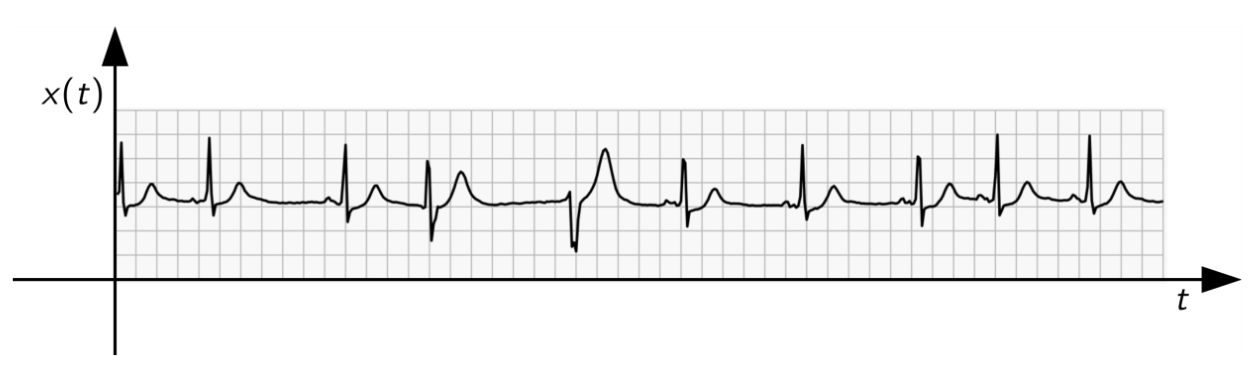
\includegraphics[scale=0.3]{../figures/audio_sig.png}
		\end{center}

		$$
		\text{Suono}(t) = \text{Ampiezza}, \quad \text{Suono} : \mathbb{R} \rightarrow \mathbb{R}
		$$

	\newpage

	\item Un'\textbf{immagine} in bianco e nero può essere rappresentata come una funzione governata dalle variabili temporali $x$, $y$:	
		\begin{center}
			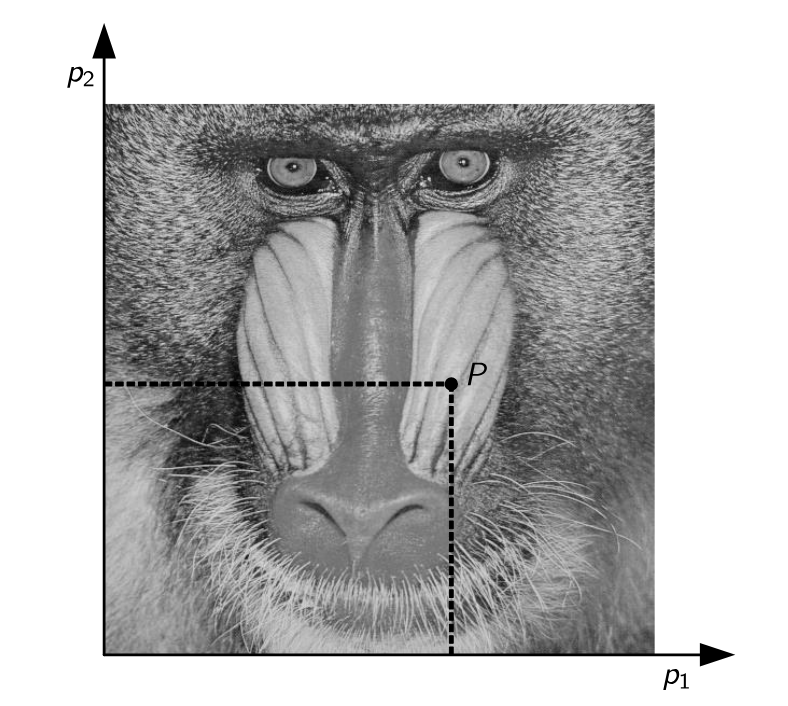
\includegraphics[scale=0.3]{../figures/img_sig.png}
		\end{center}

		$$
		\text{Immagine}(x,y) = \text{Luminosità}, \quad \text{Immagine} : \mathbb{R}^2 \rightarrow \mathbb{R}
		$$
		nel caso di funzioni a colori, dovremmo mappare i nostri pixel a triple $(r, g, b)$ (o comunque usare un qualche schema di rappresentazione del colore, cosa che solitamente richiede 3 dimensioni indipendenti), e quindi avere:
		$$
		\text{Immagine}^C(x,y) = (r, g, b), \quad \text{Immagine}^c : \mathbb{R}^2 \rightarrow \mathbb{R}^3
		$$

		Introducendo una dimensione temporale alla funzione (e restando per ora in bianco e nero), si può trasformare questo segnale $\text{Immagine}(x, y)$ in un segnale $\text{Video}(x, y, t)$:
		\begin{center}
			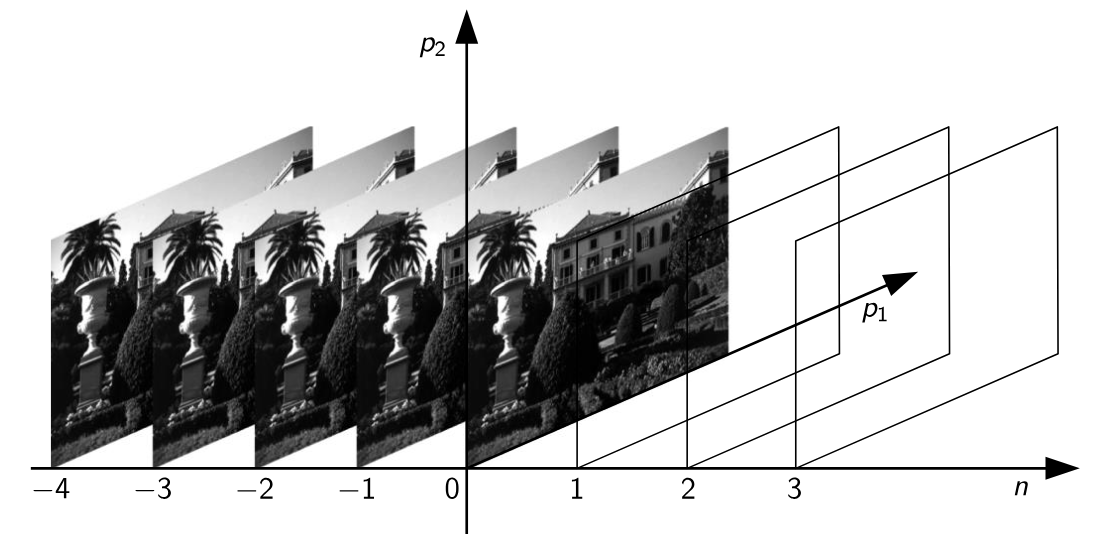
\includegraphics[scale=0.3]{../figures/video_sig.png}
		\end{center}

		$$
		\text{Video}(x,y,t) = \text{Luminosità}, \quad \text{Video} : \mathbb{R}^3 \rightarrow \mathbb{R}
		$$
\end{itemize}

\newpage

Un altra distinzione può essere fatta fra segnali \textit{analogici} e \textit{digitali}:
\begin{itemize}
	\item I segnali \textbf{analogici} sono quelli che troviamo in natura (e che abbiamo descritto finora). In questo, possono assumere la forma di segnali \textit{acustici}, segnali \textit{elettrici}, ecc... Vengono descritti da funzioni reali di variabile reale, e quindi hanno bisogno di una precisione potenzialmente infinita per poter essere resi in maniera accurata;
	\item I segnali \textbf{digitali} sono quelli che \textit{discretizziamo} campionando i segnali analogici periodicamente. Abbiamo che questo processo perde per forza informazione riguardo al segnale originale, ma è l'unico modo per gestire i segnali che vengono dal mondo esterno, all'interno dei sistemi di elaborazione digitali.
\end{itemize}

\subsubsection{Campionamento di segnali}
Descriviamo un caso reale di \textit{campionamento} di un segnale analogico, diciamo un segnale audio trasformato in segnale elettrico attraverso un \textit{trasduttore} (un \textit{microfono}), per farci un idea del tipo di procedura e delle limitazioni che incontriamo. 

\begin{center}
	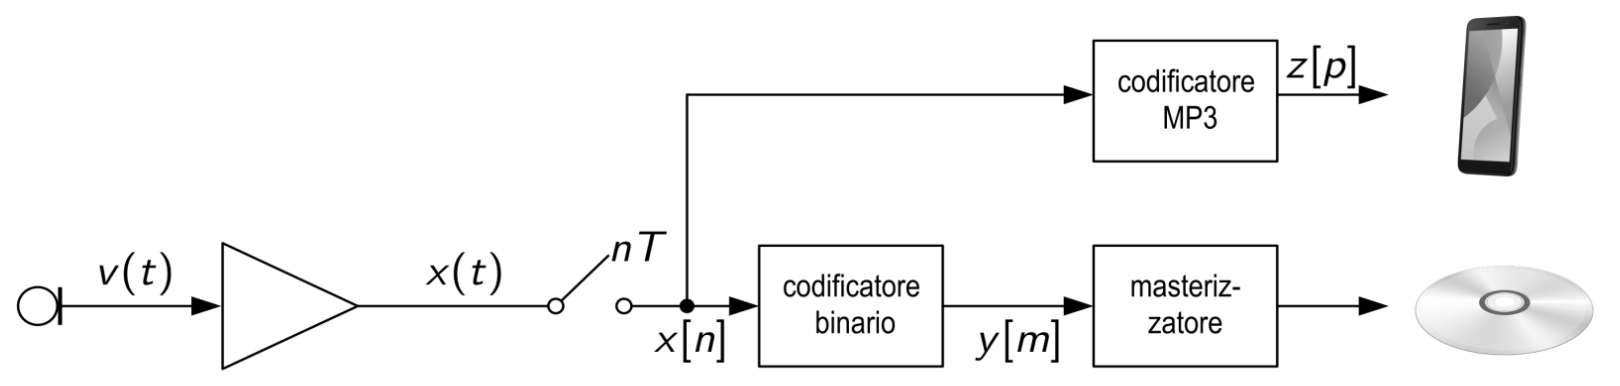
\includegraphics[scale=0.28]{../figures/sampling_intro.png}
\end{center}

\begin{enumerate}
	\item Quello che vogliamo fare è prendere, inizialmente, il segnale $v(t)$ direttamente dal \textbf{trasduttore} (microfono):
\begin{center}
	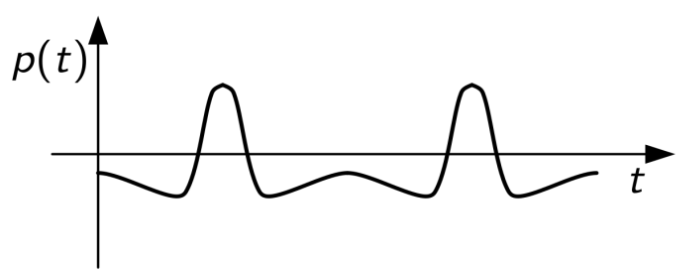
\includegraphics[scale=0.3]{../figures/sig_orig.png}
\end{center}

	\item Per avere una buona resa del segnale, sarà opportuno far passare il segnale del trasfuttore attraverso un \textbf{amplificatore} che ne aumenti l'ampiezza:
\begin{center}
	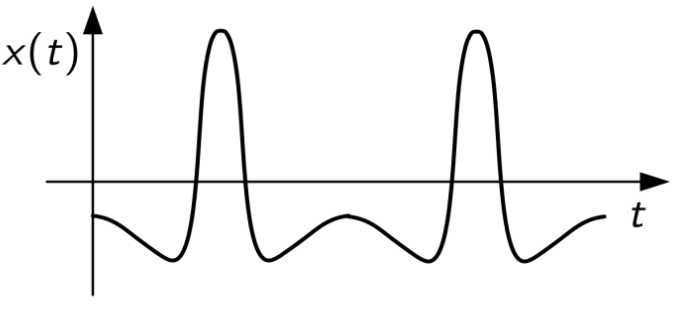
\includegraphics[scale=0.3]{../figures/sig_amp.png}
\end{center}

\newpage

	\item \textbf{Campioniamo} quindi il segnale ottenuto (che chiamiamo $x(t)$) ad intervalli regolari $T$, e cioè con un \textit{periodo} di campionamento $T$ o analogamente una \textit{frequenza} di campionamento $f = \frac{1}{T}$:
\begin{center}
	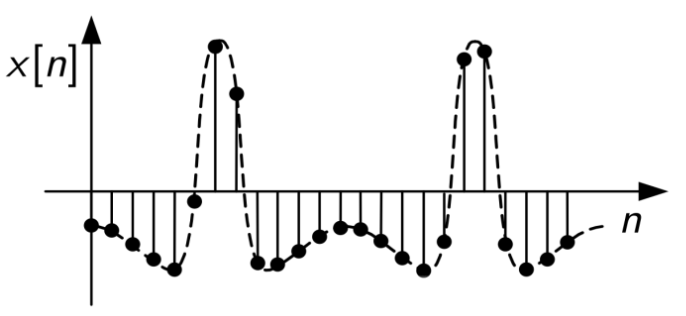
\includegraphics[scale=0.3]{../figures/sig_samp.png}
\end{center}
		Questo significherà che "registreremo" il valore di $x(t)$, per ogni naturale $n$, al tempo $nT$, ottenendo la funzione:
		$$
			x[n] = x(nT)
		$$
		di argomento naturale;
	\item Il segnale campionato potrà quindi entrare il dominio digitale ed essere codificato, masterizzato o compresso in vari modi (come si vede dalla figura).

		In particolare, il primo passo da effettuare sarà quello di codificare ogni campione (che è comunque rimasto un numero $\in \mathbb{R}$) in una codifica binaria, quindi scegliere $d$ bit (solitamente 8, 16 o 24) per rappresentare ogni campione e scrivere in una determinata porzione di memoria un vettore contenente le codifiche di tutti i campioni registrati.
	Chiamiamo il segnale così ottenuto $Y[m]$:
\begin{center}
	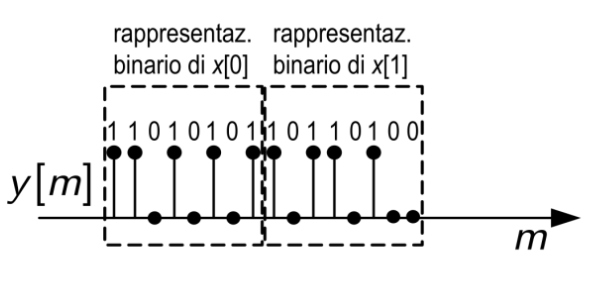
\includegraphics[scale=0.3]{../figures/sig_dig.png}
\end{center}

		Notiamo quindi di avere una doppia perdita di informazione:
		\begin{itemize}
			\item Quella ottenuta campionando il segnale ad intervalli regolari $T$, che quindi si verifica nel dominio \textit{temporale};
			\item Quella ottenuta "campionando" ancora in qualche modo le ampiezze riportandole ad un dominio:
				$$
					[-2^{(d - 1)}, 2^{(d - 1)} - 1]
				$$
				scalato sui bound dell'ampiezza del segnale campionato (solitamente negli impianti agli 0 dB del \textit{full scale} o poco più in alto). 
				Questa perdita si verifica quindi nel dominio dell'\textit{ampiezza}, e viene detta errore di \textbf{quantizzazione}.
		\end{itemize}

		Il processo di \textit{quantizzazione} dei segnali prende anche il nome di conversione \textbf{ADC} (\textit{Analog to Digital Conversion}). I dispositivi che operano la conversione ADC, come abbiamo detto, lavorano solitamente in un range che va dagli 8 ai 24 bit.
	
		\newpage

		Inoltre, possono supportare 2 tipologie principali di quantizzazione:
		\begin{itemize}
			\item Quantizzazione \textit{uniforme}: dove i valori codificati vanno linearmente con l'ampiezza; 
			\item Quantizzazione \textit{non-uniforme}: dove i valori codificati vanno in maniera non lineare con l'ampiezza. Convertitori di questo tipo sono più difficili da realizzari ma in alcune situazioni possono raggiungere fedeltà nella resa del segnale originale migliori rispetto alle controprati uniformi.
		\end{itemize}
\end{enumerate}

Come vedremo, esiste un'equazione per la frequenza di campionamento minima che ci permette di ricostruire un segnale a partire da una sua versione campionata:
$$
f = \frac{1}{T} \geq 2 B
$$
dove $B$ è la larghezza di banda del segnale originale (assunto che questo segnale abbia dominio di banda finito). Chiamiamo questo risultato teorema di \textit{campionamento di Nyquist-Shannon}. Unito alla ricostruzione del segnale originale con un operatore cosiddetto \textit{seno cardinale}, questo ci assicura che il passaggio da mondo analogico e digitale può essere fatto senza perdita di informazione. 

\subsubsection{Tipologie di segnale}
Notiamo che, nello scorso esempio, abbiamo visto diversi tipi di segnale. Possiamo individuare 2 caratteristiche ortogonali, date dalla \textbf{continuità} o meno nel dominio \textit{temporale} e nel dominio di \textit{ampiezza}:
\begin{itemize}
	\item Chiamiamo \textbf{analogici} i segnali continui nel tempo e nelle ampiezze:
\begin{center}
	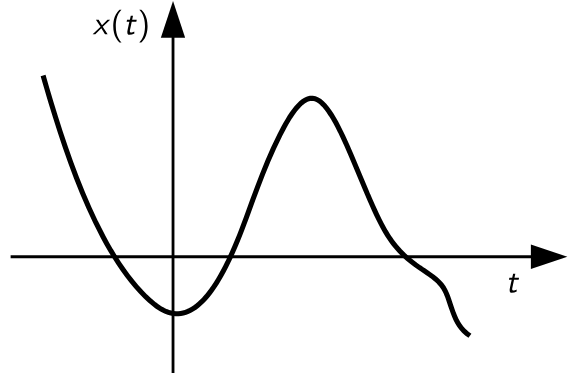
\includegraphics[scale=0.3]{../figures/anal_sig.png}
\end{center}
Questi corrispondono al segnale originale che volevamo campionare nello scorso esempio, come ai segnali elettrici campionati e poi amplificati ($v(t)$ e $x(t)$);
	\item Chiamiamo \textbf{sequenze} i segnali discontinui nel tempo e continui nelle ampiezze:
\begin{center}
	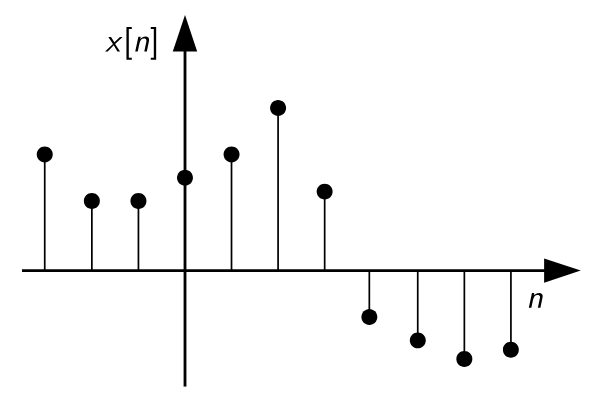
\includegraphics[scale=0.3]{../figures/seq_sig.png}
\end{center}
questi corrispondono al segnale campionato dal campionatore, cioè $x[n]$;
	\item Chiamiamo \textbf{quantizzati} i segnali continui nel tempo e discontinui nelle ampiezze:
\begin{center}
	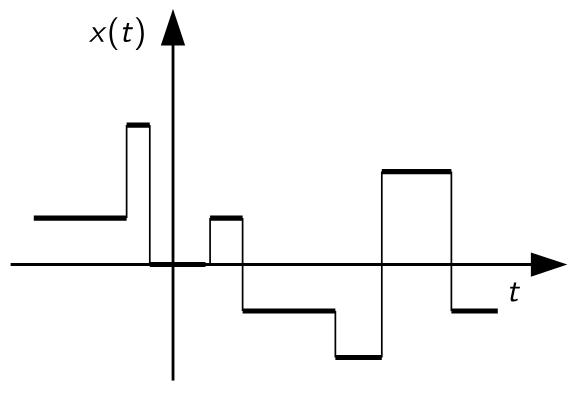
\includegraphics[scale=0.3]{../figures/quant_sig.png}
\end{center}
non abbiamo ancora visto segnali di questo tipo, ma possiamo considerarli versioni continue nel tempo delle sequenze;
	\item Infine, chiamiamo \textbf{digitali} i segnali discontinui nel tempo e nelle ampiezze:
\begin{center}
	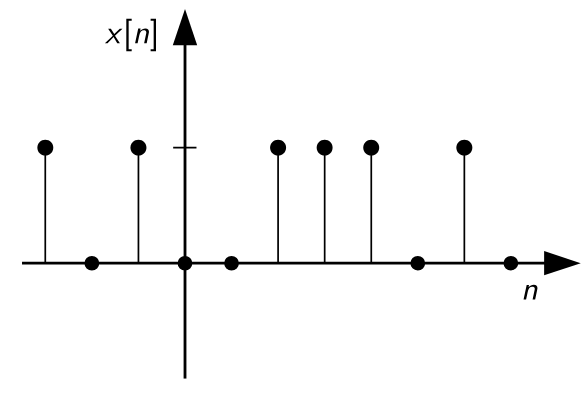
\includegraphics[scale=0.3]{../figures/dig_sig.png}
\end{center}
questi sono effettivamente i segnali come $y[n]$ che trattiamo nei sistemi di elaborazione digitale. Notiamo che, visto che ogni campione va rappresentato da una sequenza di $d$ bit, la frequenza di informazione dei segnali digitali $f_d$ e la frequenza di informazione dei corrispondenti segnali campionati $f_c$ obbedisce la relazione:
$$
f_d \geq f_c
$$
dove l'uguaglianza si ha nel caso banale in cui si rappresenta il campione con un solo bit.
\end{itemize}

\par\smallskip

\noindent
\textbf{\textsf{Sistemi di comunicazione a campionamento}}

\noindent
Possiamo quindi confrontare le nozioni finora acquisite con quanto avevevamo discusso nella prima lezione, sezione 1.2 . Avevamo infatti discusso la struttura di un \textit{sistema di comunicazione}, e viste le parti che lo costituivano operando l'elaborazione dei segnali. 
\begin{center}
	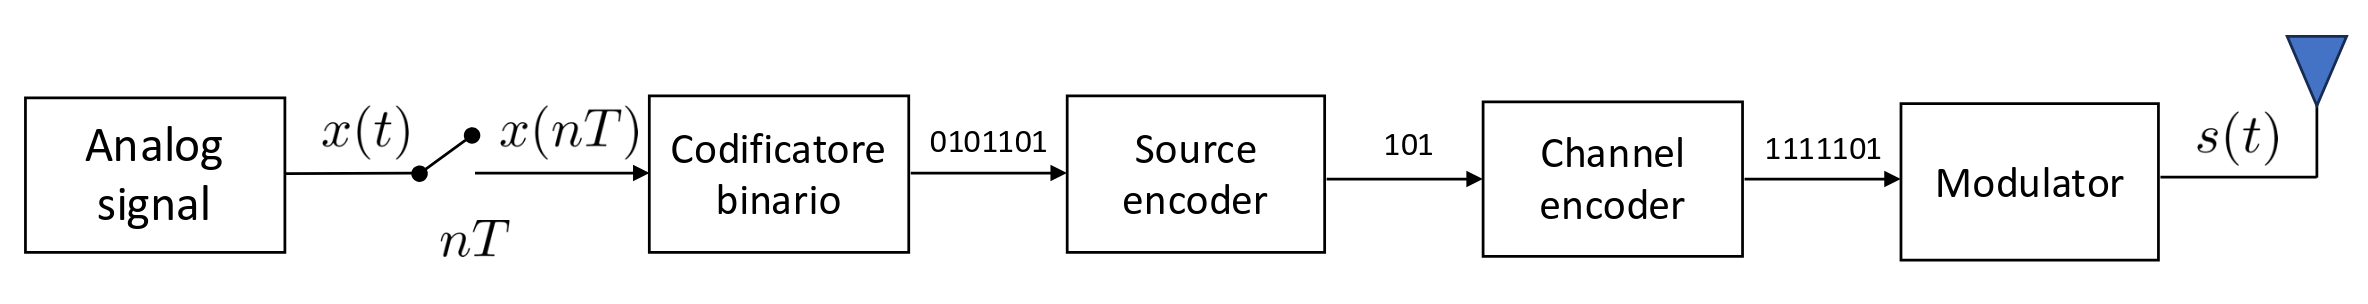
\includegraphics[scale=0.175]{../figures/sig_encode.png}
\end{center}

\newpage

Adesso possiamo dare una descrizione reale di ciò che accade ai segnali nel corso della \textit{pipeline} di un \textbf{trasmettitore} che attraversano:
\begin{enumerate}
	\item Prima di tutto, il segnale analogico (che può essere acustico, elettrico, elettrico convertito da analogico, ecc...) deve essere \textbf{campionato} ad intervalli regolari $T$. Quandi si effettua il campionamento, la frequenza dell'informazione (cioè la banda) diminuisce (e si perde informazione);
	\item Il segnale dovrà quindi essere codificato (o meglio dovranno essere codificati i campioni) attraverso un \textbf{codificatore binario}. Come avevamo detto, ogni campione richiede più bit, per cui la larghezza di banda dovrà aumentare;
	\item Segue il \textbf{source encoder}, già visto in 1.2, che avrà l'obiettivo di comprimere il segnale ottimizzandone la rappresentazione digitale, e quindi diminuire la larghezza di banda. Per far questo notiamo che sfruttava la \textit{ridondanza} intrinseca del segnale, rimuovendola;
	\item Segue il \textbf{channel encoder}, anche questo già visto in 1.2, che dovrà preparare il segnale alla trasmissione sul mezzo e quindi solitamente aumenterà la larghezza di banda introducendo \textit{ridondanza} utile al rilevamento degli errori;
	\item Infine il segnale preparato dal channel encoder potrà essere messo sul mezzo di trasmissione dal \textbf{modulatore}. Molto probabilmente, sul mezzo vero e proprio il segnale assumerà di nuovo una forma analogica (ad esempio un segnale elettrico su un cavo in rame).
\end{enumerate}

Dall'altro capo del sistema ci sarà un apparato \textbf{ricevitore} che dovrà svolgere tutte queste operazioni al contrario, ricostruendo quindi il segnale analogico originale (o molto più probabilmente una sua rappresentazione più o meno accurata).

\subsection{Segnali complessi}
Iniziamo a parlare di segnali \textit{complessi}, cioè rappresentati da due valori in evoluzione nel tempo o su un altra grandezza $a(t)$ e $b(t)$. Rappresentiamo questo segnale come un numero complesso $\in \mathbb{C}$:
$$
z(t) = a(t) + i b(t) = c(t)e^{i \theta(t)}
$$

Essendo questo segnale una funzione complessa ad argomento reale, possiamo applicare le proprietà viste in 1.3, in particolare riguardo ai numeri complessi. Definiamo inoltre le operazioni di integrale e derivata di tale segnale:
\begin{itemize}
	\item \textit{Integrale}: 
$$
\int z(t) \, dt = \int a(t) \, dt + i \int b(t) \, dt
$$
	\item \textit{Derivata}:
$$
\frac{d \, z(t)}{dt} = \frac{d \, a(t)}{a(t)} + i \frac{d \, b(t)}{b(t)}
$$
\end{itemize}

\par\smallskip

\noindent
\textbf{\textsf{Potenza}}

\noindent
Se si parla di valori complessi, è utile dare una qualche nozione di \textbf{potenza}. L'origine più intuitiva di un concetto di potenza è il dominio dei circuiti elettrici, dove la potenza dissipata su un componente passivo come un resistore è uguale a:
$$
P(t) = R I^2(t)
$$

Questa legge è applicabile in astratto, per cui dato un qualunque segnale $x(t)$ (qui era $I(t)$) vale:
\begin{definition}{Potenza istantanea}
La \textbf{potenza istantanea} di un segnale $x(t)$ è proporzionale al suo quadrato:
$$
P(t) = |x(t)|^2
$$
\end{definition}

\par\smallskip

\noindent
\textbf{\textsf{Energia}}

\noindent
Data una definizione di \textit{potenza} espressa in funzione dell'energia:
$$
P = \frac{E}{t}
$$
cioè energia $E$ su tempo $t$, è appunto semplice dare una definizione di \textbf{energia} dissipata su un certo periodo di tempo. Questa, dagli strumenti di analisi, potrà essere calcolata come l'integrale:
$$
E_{x_T} = \int_{t_0}^{t_1} P(t) \, dt = \int_{t_0}^{t_1} |x(t)|^2 \, dt
$$
su un certo intervallo temporale $[t_0, t_1]$.

Molto più spesso, vorremo calcolare l'energia da $-\infty$ a $+\infty$ di un segnale, cioè quella su tutto $t \in \mathbb{R}$. Per fare ciò, prendiamo l'intervallo:
$$
[t_0, t_1] = \left[-\frac{T}{2}, \frac{T}{2}\right] 
$$
per una qualche dimensione di \textit{finestra} $T$, cioè la finestra centrata sull'origine, da cui otteniamo la nuova espressione di $E_{x_T}$:
$$
E_{x_T} = \int_{-\frac{T}{2}}^{\frac{T}{2}} P(t) \, dt = \int_{-\frac{T}{2}}^{\frac{T}{2}} |x(t)|^2 \, dt
$$
a questo punto basterà prende il limite per $T \rightarrow + \infty$ per ottenere:
\begin{definition}{Energia}
L'\textbf{energia} espressa sul dominio $\mathbb{R}$ da un segnale $x(t)$ è espressa come:
$$
E_x = \lim_{T \rightarrow + \infty} E_{x_T} = \lim_{T \rightarrow + \infty} \int_{-\frac{T}{2}}^{\frac{T}{2}} |x(t)|^2 \, dt
$$
\end{definition}
questa sarà la definizione di energia complessiva che useremo da qui in poi.

\par\smallskip

\noindent
\textbf{\textsf{Segnale troncato}}

\noindent
Vediamo un dettaglio, prendiamo il segnale:
$$
x_T (t) = \{ t_0 < t < t_1 : \, x(t), \, 0 \text{ altrimenti} \}
$$
come la versione \textbf{troncata} sull'intervallo $[t_0, t_1]$ del segnale $x(t)$. Calcolare l'energia del segnale $x(t)$ sull'intervallo $[t_0, t_1]$ equivarrà a calcolare l'energia da $-\infty$ a $+\infty$ del segnale troncato. Vedremo subito come queste definizioni ci sono utili nella definizione di potenza media.

\par\smallskip

\noindent
\textbf{\textsf{Potenza media}}

\noindent
Una volta che abbiamo un'idea di \textit{energia} dissipata o erogata nel tempo, possiamo definire la \textbf{potenza media} su un \textit{intervallo} (altresì dissipata o erogata nel tempo) come:
$$
P_{x_T} = \frac{E_{x_T}}{t_1 - t_0} \, \quad E_{x_T} = \int_{t_0}^{t_1} x^2 (t) \, ds
$$
Spostiamoci sull'intervallo:
$$
[t_0, t_1] = \left[-\frac{T}{2}, \frac{T}{2}\right] 
$$
che è cio che avevamo fatto per ricavare l'energia complessiva su $\mathbb{R}$. Questo diventa quindi:
$$
P_{x_T} = \frac{E_{x_T}}{T} \, \quad E_{x_T} = \int_{-\frac{T}{2}}^{\frac{T}{2}} x^2 (t) \, dt
$$
di cui prendiamo il limite per $T \rightarrow + \infty$ per ottenere:
\begin{definition}{Potenza media}
La \textbf{potenza media} espressa sul dominio $\mathbb{R}$ da un segnale $x(t)$ è espressa come:	
$$
P_{x} = \lim_{T \rightarrow + \infty} P_{x_T} = \lim_{T \rightarrow + \infty} \frac{E_{x_T}}{T} = \lim_{T \rightarrow + \infty} \frac{1}{T} \int_{-\frac{T}{2}}^{\frac{T}{2}} x^2 (t) \, dt 
$$
\end{definition}
Generalmente, da qui in poi useremo questa definizione per riferirci alla potenza dei segnali. 

Osserviamo che:
\begin{itemize}
	\item Un segnale ad energia \textit{finita} ha potenza media \textit{nulla};
	\item Un segnale a potenza media \textit{finita} ha energia \textit{infinita}.
\end{itemize}

\par\smallskip

Vediamo quindi alcuni segnali di esempio, calcolandone la potenza media e l'energia.

\begin{itemize}
	\item \textbf{\textsf{Segnale costante}} \\
Consideriamo un primo segnale banale, cioè il segnale \textit{costante}:
$$
x(t) = 1
$$

In questo caso l'\textit{energia} è infinita e la \textit{potenza media} costante unitaria, in accordo con le due regole enunciate prima. Questo è di facile derivazione:
$$
E_x = \lim_{T \rightarrow + \infty} \int_{-\frac{T}{2}}^{\frac{T}{2}} |1|^2 \, dt =  \lim_{T \rightarrow + \infty} T = + \infty
$$
$$
P_x = \lim_{T \rightarrow + \infty} \frac{1}{T} \int_{-\frac{T}{2}}^{\frac{T}{2}} |1|^2 \, dt =  \lim_{T \rightarrow + \infty} \frac{1}{T} T = 1 
$$

	\item \textbf{\textsf{Segnale gradino}} \\
Il segnale \textit{gradino} è un segnale che vale zero per $t < 0$ e una costante per $t >= 0$. Si indica con $u(t)$:
\[
	x(t) = 
	\begin{cases}
		0, \quad t < 0 \\
		\frac{1}{2}, \quad t = 0 \\
		1, \quad t > 0
	\end{cases}
\]
Viene detto anche gradino di \textit{Heaviside}, per cui si indica talvolta con $h(t)$.

L'\textit{energia} del segnale gradino vale infinito mentre la \textit{potenza media} è costante, uguale ad $\frac{1}{2}$ (in accordo con quanto detto prima). Deriviamo:
$$
E_x = \lim_{T \rightarrow + \infty} \int_{-\frac{T}{2}}^{\frac{T}{2}} |x(t)|^2 \, dt = \lim_{T \rightarrow + \infty} \left( \int_{-\frac{T}{2}}^0 0 \, dt + \int_0^{\frac{T}{2}} 1 \, dt \right) = \lim_{T \rightarrow + \infty} \frac{T}{2} = + \infty
$$
$$
P_x = \lim_{T \rightarrow + \infty} \frac{1}{T} \int_{-\frac{T}{2}}^{\frac{T}{2}} |x(t)|^2 \, dt = \lim_{T \rightarrow + \infty} \frac{1}{T} \left( \int_{-\frac{T}{2}}^0 0 \, dt + \int_0^{\frac{T}{2}} 1 \, dt \right) = \lim_{T \rightarrow + \infty} \frac{1}{T} \frac{T}{2} = \frac{1}{2} 
$$

	\item \textbf{\textsf{Segnale esponenziale monolatero}} \\ 
Il segnale \textit{esponenziale monolatero} vale zero per $t < 0$ e decade in maniera esponenziale per $t > 0$, cioè:
$$
x(t) = e^{-\frac{t}{\tau}} \cdot u(t)
$$
secondo un certo \textit{tempo caratteristico} $\tau$. Notiamo di aver usato il segnale gradino nella definizione.

Questo sarà il primo segnale che vediamo ad \textit{energia} finita, in quanto in particolare vale $\frac{1}{2}$. Ne segue naturalmente che la \textit{potenza media} è nulla. Deriviamo prima l'energia:
$$
E_x = \lim_{T \rightarrow + \infty} \int_{-\frac{T}{2}}^{\frac{T}{2}} \left| e^{-\frac{t}{\tau}} \cdot u(t) \right|^2 \, dt = \lim_{T \rightarrow + \infty} \int_0^{\frac{T}{2}} e^{-\frac{2t}{\tau}}  \, dt = \lim_{T \rightarrow + \infty} - \frac{\tau}{2} e^{-\frac{2t}{\tau}} \Big|^{\frac{T}{2}}_0 =
$$
$$
= \lim_{T \rightarrow + \infty} \left( - \frac{\tau}{2} e^{-\frac{T}{\tau}} + \frac{\tau}{2} e^0 \right) = \frac{\tau}{2} < + \infty
$$
e quindi la potenza media:
$$
P_x = \lim_{T \rightarrow + \infty} \frac{1}{T} \int_{-\frac{T}{2}}^{\frac{T}{2}} \left| e^{-\frac{t}{\tau}} \cdot u(t) \right|^2 \, dt = \lim_{T \rightarrow + \infty} \frac{1}{T} \int_0^{\frac{T}{2}} e^{-\frac{2t}{\tau}}  \, dt = \lim_{T \rightarrow + \infty} \frac{1}{T} \left( - \frac{\tau}{2} e^{-\frac{2t}{\tau}} \Big|^{\frac{T}{2}}_0 \right) =
$$
$$
= \lim_{T \rightarrow + \infty} \frac{1}{T} \left( - \frac{\tau}{2} e^{-\frac{T}{\tau}} + \frac{\tau}{2} e^0 \right) = \lim_{T \rightarrow + \infty} \frac{1}{T} \frac{\tau}{2} = 0
$$

\item \textbf{\textsf{Impulso rettangolare}} \\
Vediamo come ultimo segnale l'\textit{impulso rettangolare}. Questo si può intendere come la funzione:
$$
x(t) = 
\begin{cases}
	1, \quad |t| < \frac{\tau}{2} \\
	\frac{1}{2}, \quad |t| = \frac{\tau}{2} \\
	0, \quad |t| > \frac{\tau}{2}
\end{cases}
$$
cioè il gradino di altezza 1 centrato attorno all'origine, di durata $\tau$.

Di questa funzione si ha che l'energia, come per il segnale esponenziale monolatero, è finita. Segue che la potenza è nulla. Deriviamo: 
$$
E_x = \lim_{T \rightarrow + \infty} \int_{-\frac{T}{2}}^{\frac{T}{2}} |x(t)|^2 \, dt = \lim_{T \rightarrow + \infty} \int_{-\frac{\tau}{2}}^{\frac{\tau}{2}} 1 \, dt = \lim_{T \rightarrow + \infty} \tau = \tau
$$
$$
P_x = \lim_{T \rightarrow + \infty} \frac{1}{T} \int_{-\frac{T}{2}}^{\frac{T}{2}} |x(t)|^2 \, dt = \lim_{T \rightarrow + \infty} \frac{1}{T} \int_{-\frac{\tau}{2}}^{\frac{\tau}{2}} 1 \, dt = \lim_{T \rightarrow + \infty} \frac{1}{T} \tau = 0
$$
che nuovamente è in accordo con le regole enunciate prima di relazione fra energia e potenza. 

\item \textbf{\textsf{Segnale periodico}} \\
Consideriamo quindi il classico segnale \textit{periodico}. In generale, chiamiamo \textit{periodico} qualsiasi segnale che obbedisce la relazione:
$$
x(t) = x(t + \tau), \quad \forall t \in \mathbb{R}
$$
per un certo valore $\tau$ detto \textbf{periodo}. Chiamiamo l'opposto del periodo $\tau$ \textbf{frequenza} $f$:
$$
f = \frac{1}{\tau}
$$
In generale, per un segnale periodico vale riguardo alla potenza media:
$$
P_x = \frac{1}{\tau} \int_{-\frac{\tau}{2}}^{\frac{\tau}{2}} | x(t) |^2 \, dt
$$
Riguardo all'energia $E_x$, invece, abbiamo che:
\begin{itemize}
	\item Se la potenza media $P_x$ è nulla, lo è anche l'energia $E_x$;
	\item Se la potenza media $P_x$ è $\neq o$, l'energia $E_x$ è infinita.
\end{itemize}

Prendiamo come esempio il classico segnale \textit{sinusoidale}, nella sua forma più generale:
$$
x(t) = A \sin(\omega t + \phi) = A \sin(2 \pi f t + \phi) = A \sin\left( \frac{2 \pi}{\tau} t + \phi \right)
$$
dove:
\begin{itemize}
	\item $A$ è l'\textit{ampiezza} del segnale;
	\item $\omega$ è la \textit{pulsazione} del segnale;
	\item $\phi$ è lo \textit{scostamento di fase} del segnale;
	\item $f$ e $\tau$ sono le già viste frequenza e periodo del segnale.
\end{itemize}
Fra pulsazione, frequenza e periodo vale:
$$
\omega = 2 \pi f = \frac{2 \pi}{\tau}, \quad f = \frac{\omega}{2\pi}, \quad \tau = \frac{2\pi}{\omega}
$$

Calcoliamo quindi la \textit{potenza media} della funzione sinusoidale (per la cosinusoidale vale la stessa cosa). Prendiamo per semplicità $\phi = 0$, cioè scostamento di fase nullo (al limite si può sempre reintrodurre). Avremo quindi:
$$
P_x = \frac{1}{\tau} \int_{-\frac{\tau}{2}}^{\frac{\tau}{2}} \left| A \sin \left( \frac{2 \pi}{\tau} t \right) \right|^2 \, dt = \frac{A^2}{2 \tau} \left( \int_{-\frac{\tau}{2}}^{\frac{\tau}{2}} 1 \, dt - \int_{-\frac{\tau}{2}}^{\frac{\tau}{2}} \cos\left( \frac{4\pi}{\tau} t \right)  \, dt \right) = \frac{A^2}{2\tau} \cdot \tau = \frac{A^2}{2}
$$
dove l'integrale:
$$
\int_{-\frac{\tau}{2}}^{\frac{\tau}{2}} \cos \left( \frac{4 \pi}{\tau} t \right) \, dt = 0
$$
in quanto i confini di integrazione $[-\frac{\tau}{2}, \frac{\tau}{2}]$ corrispondono col periodo di $\cos \left( \frac{4 \pi}{\tau} t \right)$, per cui avremo un numero uguale di oscillazioni sopra e sotto l'asse delle ascisse (e quindi somma zero).

Quindi la potenza del segnale sinusoidale non dipende nè da $\omega$, né da $\phi$, ed è diversa da 0. Segue che l'\textit{energia} è infinta. In ogni caso, quando si parla di segnali periodici non nulli, sarà conveniente riferirci alle potenze piuttosto che alle energie.
\end{itemize}

\end{document}
